\subsubsection{Traduzione delle espressioni in LLVM-IR}
Come già detto nel capitolo di presentazione dell'LLVM-IR ad alto livello, le variabili in LLVM-IR sono 
solo simboli a cui sono associati dei valori, e non hanno un vero e proprio indirizzo di memoria. Per rappresentare 
una variabile in Basalt utilizzando LLVM-IR, è necessario avere due oggetti distinti, uno corrispondente al valore 
della variabile e uno corrispondente al suo indirizzo di memoria. Si utilizzerà dunque la seguente struct per modellare 
una generica espressione Basalt tradotta in LLVM-IR:

\vspace{0.5cm}
\begin{lstlisting}[frame=single]
struct TranslatedExpression {
    llvm::Value* value;
    llvm::Value* address;
};
\end{lstlisting}
\vspace{0.5cm}

Si consideri l'espressione Basalt corrispondente al solo identifier \texttt{x}, e si assuma che tale identifier corrisponda 
ad una variabile intera con valore 6 allocata ad indirizzo di memoria \texttt{0xF5FAC43D}. La sua traduzione in una \texttt{TranslatedExpression} 
avrebbe la forma:

\vspace{0.3cm}
\begin{figure}[H]
    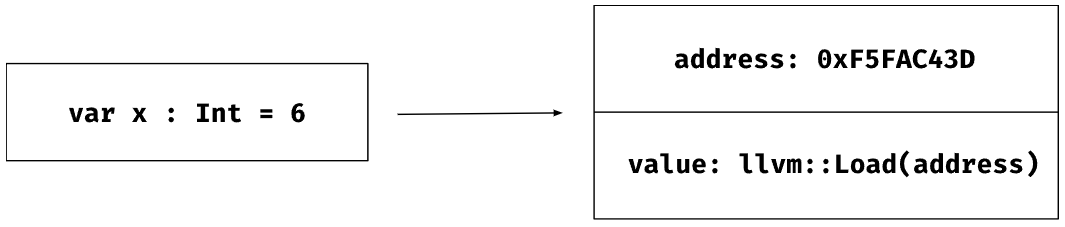
\includegraphics[width=\textwidth]{../../Assets/LLVMExpr1}
    \caption{Traduzione di un identifier in LLVM-IR}
\end{figure}
\vspace{0.3cm}

Si noti che non ogni \texttt{TranslatedExpression} ha un indirizzo di memoria associato, ad esempio l'espressione \texttt{2}
sarebbe tradotta come segue: \\

\vspace{0.3cm}
\begin{figure}[H]
    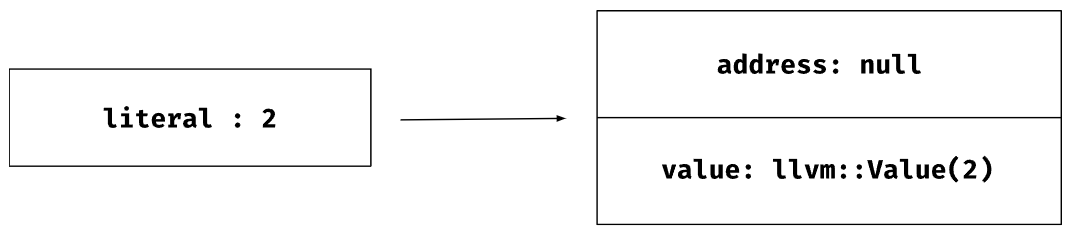
\includegraphics[width=\textwidth]{../../Assets/LLVMExpr2}
    \caption{Traduzione di una literal in LLVM-IR}
\end{figure}
\vspace{0.3cm}

\newpage

La traduzione dell'operatore unario di referenziazione (\texttt{\&}) è un po' più complessa, in quanto è necessario
tradurre l'operando in una \texttt{TranslatedExpression} e applicare ad essa una trasformazione per ottenere una nuova 
\texttt{TranslatedExpression} che rappresenti l'indirizzo di memoria dell'operando. Si consideri l'espressione \texttt{\&x}, essa
sarebbe dunque tradotta come segue: \\

\vspace{0.3cm}
\begin{figure}[H]
    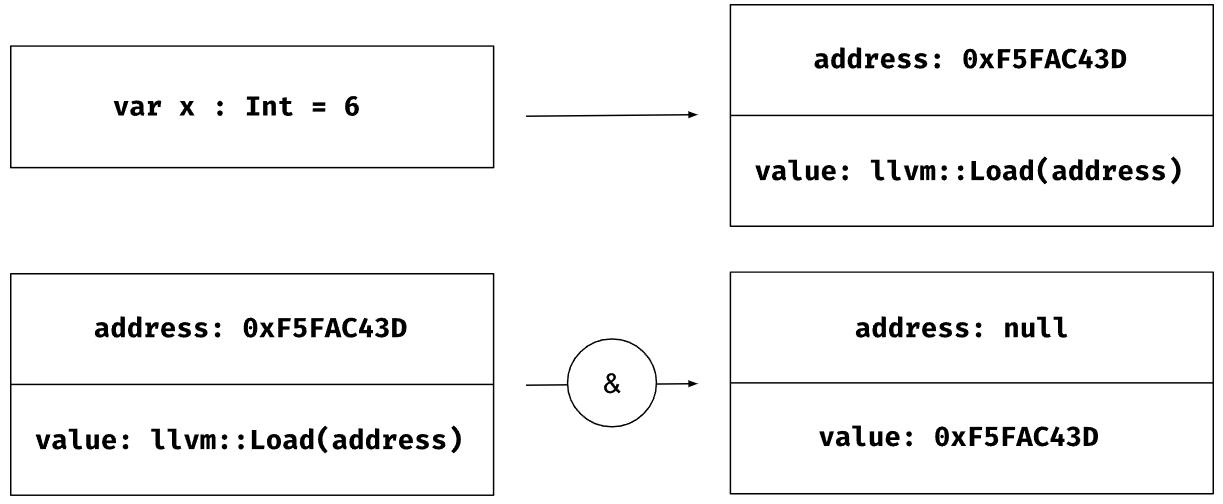
\includegraphics[width=\textwidth]{../../Assets/LLVMExpr3}
    \caption{Traduzione di una referenziazione in LLVM-IR}
\end{figure}
\vspace{0.3cm}

Una dereferenziazione, così come la dereferenziazione (\texttt{\#}), è un'operatore unario, e come tale, richiede di essere 
tradotto mediante la trasformazione della \texttt{TranslatedExpression} che rappresenta il suo operando. Si consideri
l'espressione \texttt{\#y}, dove y è un puntatore ad intero. Essa sarebbe tradotta come segue: \\

\vspace{0.3cm}
\begin{figure}[H]
    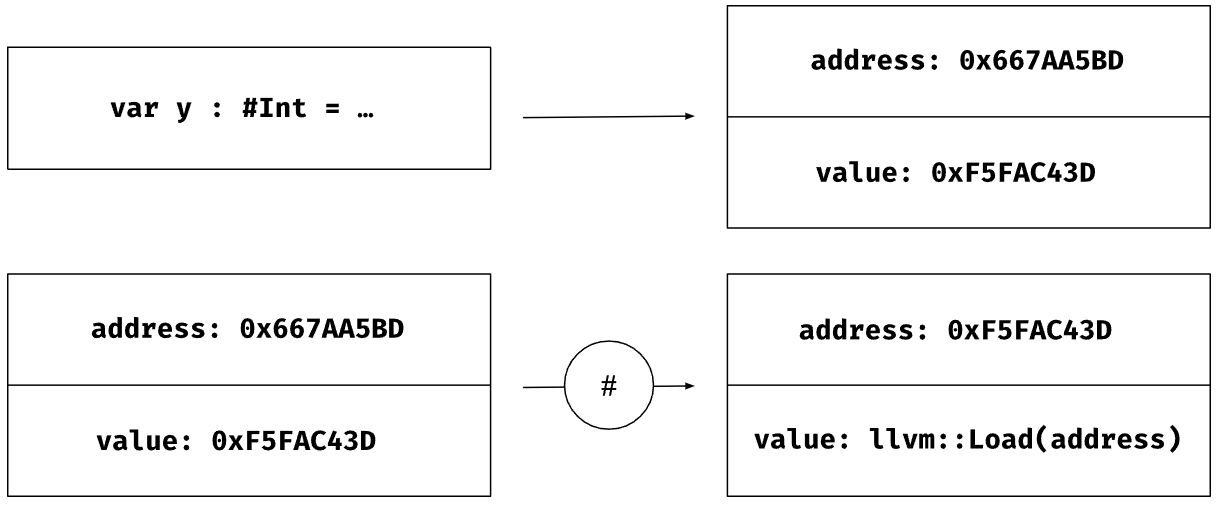
\includegraphics[width=\textwidth]{../../Assets/LLVMExpr4}
    \caption{Traduzione di una dereferenziazione in LLVM-IR}
\end{figure}
\vspace{0.3cm}

\newpage

Un generico operatore richiede la traduzione dei suoi operandi in \texttt{TranslatedExpression}, e la
successiva applicazione di una qualche fuzione dell'API di LLVM ai valori di tutte le \texttt{TranslatedExpression} ottenute. Si consideri
l'espressione \texttt{a + b}, essa sarebbe tradotta come segue: \\

\vspace{0.3cm}
\begin{figure}[H]
    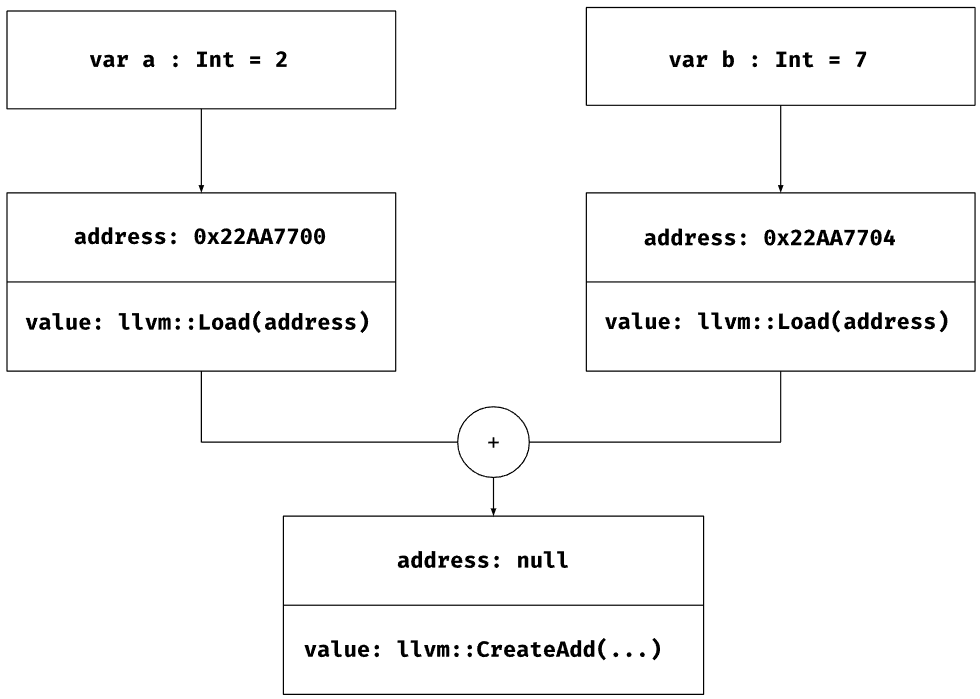
\includegraphics[width=\textwidth]{../../Assets/LLVMExpr5}
    \caption{Traduzione di una somma in LLVM-IR}
\end{figure}
\vspace{0.3cm}

Lo stesso vale anche per operatori unari come l'operatore di negazione logica (\texttt{!}). Le espressioni 
di tipo chiamata a funzione, operatore \texttt{as} ed operatore \texttt{is} sono trattate in dettaglio 
nelle sezioni successive del documento. \\

Un'array literal viene tradotta come un'allocazione di memoria, seguita da una serie di assegnazioni
ai singoli elementi dell'array. L'optimization engine di LLVM si occuperà di effettuare l'\textit{inlining}
delle assegnazioni, se possibile, o addirittura di rimuovere del tutto l'allocazione ed utilizzerà direttamente 
i valori la dove servono. Ovviamente, ciò è possibile solo se l'array literal viene usata in contesti 
dove i valori sono noti a priori e/o sono noti a priori gli indici ai quali saranno effettuate letture. \\

\newpage